% ======================================================================
% Section 3 — Proposed Method (revised from submitted_version)
% Framing: GSL for traffic prediction; multi-lag + Mix extend the same idea.
% ======================================================================
\section{The Proposed Method: Estimating the Adjacency Matrix with Graph Structure Learning}\label{sec:method}

In both GCN \citep{kipf2017semi} and T-GCN \citep{zhao2019t}, the adjacency
matrix $\mathbf{A}$ that describes spatial relationships among sensors is
typically predefined from urban planning or road-network information. Here we
estimate $\mathbf{A}$ from traffic data, which is known as \emph{graph
structure learning} (GSL) \citep{Chen2022}. The goal is to obtain a graph
representation that reflects dependency structure present in the observed
series rather than structure imposed solely by physical proximity.

\subsection{Motivation}\label{sec:method-motivation}

In a typical urban traffic network, spatial proximity of roads need not
coincide with statistical dependence among their speeds. Distant segments can
be strongly correlated through shared demand, while adjacent segments can be
weakly related. Propagation delay is also relevant: association between two
sensors may appear only at particular temporal lags. Estimating the adjacency
directly from the data allows the forecasting model to aggregate from
neighbors defined by observed co-movement rather than only by the map.

\begin{figure}[t]
\centering
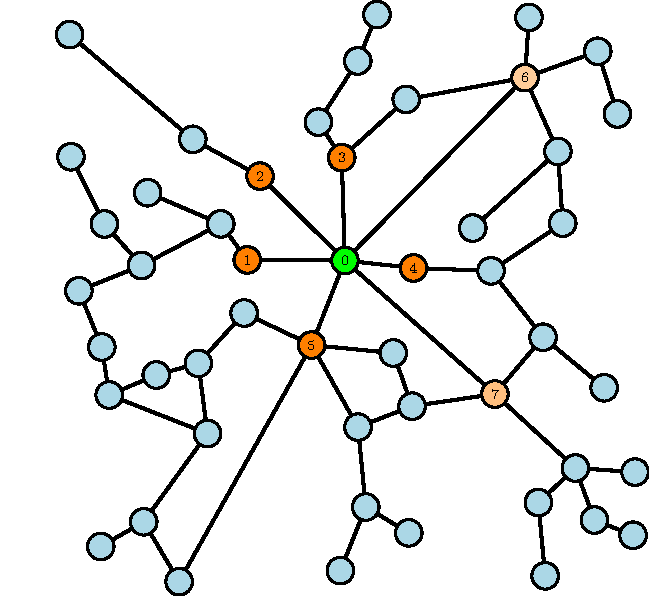
\includegraphics[width=0.55\linewidth]{dummy-network.pdf}
\caption{Conceptual two-dimensional traffic network. Association between a
target node (green) and other nodes depends not only on spatial proximity
(lighter color indicates larger distance) but also on topology and travel
time. The learned adjacency aims to reflect such data-driven associations
rather than geographic distance alone.}
\label{dummy-network-main-idea}
\end{figure}

Figure~\ref{dummy-network-main-idea} illustrates a stylized network related
to Figure~\ref{fig:GCN}. Three points motivate data-driven adjacency:
(i) nearby nodes may share more immediate co-movement than distant ones, but
this need not hold for every pair; (ii) associations between distant nodes
may occur at longer lags; (iii) some physically adjacent links may carry
little predictive information for the target sensor. By learning
$\mathbf{A}$ from traffic observations, the model can place edges according
to estimated dependency rather than geographic distance alone.

Throughout this section, $\mathbf{A}\in\{0,1\}^{N\times N}$ denotes the
binary adjacency supplied to the forecasting backbone
(Eqs.~\eqref{eq:gcn-layer}--\eqref{eq:two-layer-gcn}), and
$W\in\mathbb{R}^{d\times d}$ denotes the continuous coefficient matrix
estimated by the graph-learning procedure. The two symbols are not
interchangeable: $W$ is the estimator's internal representation; $\mathbf{A}$
is the thresholded graph used by GCN or T-GCN.

\subsection{Integration of Learned Structure with Temporal Modeling}\label{sec:method-integration}

The overall pipeline separates three stages:
\begin{itemize}
\item \textbf{Graph estimation (GSL).} A static adjacency is estimated from
training traffic data (contemporaneous or multi-lag constructions below).
\item \textbf{Normalization.} Every adjacency used in this paper ---
physical, identity (graph-free control), and learned --- is passed through
the same GCN-style operator
\begin{equation}\label{eq:norm}
\hat{\mathbf{A}}
=\tilde{\mathbf{D}}^{-1/2}\,\tilde{\mathbf{A}}^{\top}\,\tilde{\mathbf{D}}^{-1/2},
\qquad
\tilde{\mathbf{A}}=\mathbf{A}+\mathbf{I},\quad
\tilde{D}_{ii}=\sum_j\tilde{A}_{ij}.
\end{equation}
For the identity adjacency this reduces to $\hat{\mathbf{A}}=\mathbf{I}$, so
the graph-free control differs only in the absence of off-diagonal structure.
\item \textbf{Forecasting backbone.} GCN or T-GCN consumes the normalized
operator. The learned graph is \emph{static} after estimation: it is fitted
once on the training split. Temporal variation in the forecast is modeled by
the recurrent backbone (and, in one variant, by a gate that selects among
fixed lag-specific graphs); the edge set itself does not change over time.
\end{itemize}

Two reference adjacencies accompany the learned graphs in all experiments:
the \emph{physical} road-network graph (standard T-GCN/GCN baseline) and a
\emph{graph-free} identity control (T-GCN-NoSpatial / GCN-NoSpatial). The
latter is required to measure whether learned structure adds value beyond
removing a possibly harmful dense proximity graph.

\subsection{Continuous Optimization for Graph Structure Learning}\label{sec:method-notears}

Score-based GSL seeks a weighted adjacency that fits the data under a
structural equation model (SEM). Following the continuous formulation of
\citet{zheng2018dags}, let $\mathbf{X}\in\mathbb{R}^{n\times d}$ be a data
matrix with $n$ observations of $d$ variables. In traffic, rows of
$\mathbf{X}$ are time indices and columns are sensors. Instead of searching
the discrete DAG space, one optimizes over
$W\in\mathbb{R}^{d\times d}$ with a smooth acyclicity constraint
\citep{zheng2018dags}:
\begin{align}
\label{eq:main:idea}
\begin{aligned}
\min_{W} &\quad \score(W)\\
\text{subject to} &\quad h(W)=0,
\end{aligned}
\end{align}
where $\score$ measures data fit and $h$ vanishes exactly on acyclic graphs.
NOTEARS uses
\begin{equation}\label{eq:def:h}
h(W)=\tr\bigl(e^{W\circ W}\bigr)-d,
\end{equation}
with gradient
$\grad h(W)=(e^{W\circ W})^{\!\top}\circ 2W$, and solves the program with an
augmented Lagrangian
\begin{equation}
L^{\rho}(W,\alpha)=\score(W)+\tfrac{\rho}{2}\,|h(W)|^{2}+\alpha\,h(W).
\end{equation}
After optimization, a binary support is obtained by absolute-magnitude
thresholding, $\widehat{W}=W\circ\mathbf{1}(|W|>\omega)$. Algorithmic details
appear in \citep{zheng2018dags}.

\paragraph{Estimator used in this paper (DAGMA).}
In the experiments we use \textbf{DAGMA} \citep{Bello2024DAGMA}, which
replaces the NOTEARS trace-exponential constraint with a log-determinant
acyclicity characterization suitable for efficient constrained optimization,
together with a linear SEM score ($\ell_2$ reconstruction loss) and an
$\ell_1$ sparsity penalty $\lambda_1\lVert W\rVert_1$. Acyclicity is an
\emph{optimization regularizer} of the estimator. We interpret the learned
graph as a statistical dependency structure under the linear SEM assumptions,
not as a causal traffic model. DAGMA is applied in two related ways:
a \emph{contemporaneous} construction (single graph among sensors;
Section~\ref{sec:gsl_contemp}) and a \emph{multi-lag} construction
(lag-specific blocks; Section~\ref{sec:gsl_multilag}).

\subsection{Contemporaneous Graph Learning (GSL and cGSL)}\label{sec:gsl_contemp}

The contemporaneous construction is a single learned graph among the $N$
sensors from simultaneous observations --- the direct analogue of the
original GSL-for-traffic idea.

\paragraph{Input and fit.}
DAGMA is fitted to the training-split snapshot matrix
\[
\mathbf{X}=\mathrm{train\_norm}[\,0::\mathrm{PH}\,],
\]
i.e.\ every $\mathrm{PH}$-th training row (one simultaneous vector of $N$
sensor speeds per row; no lag blocks). For Los-loop the row counts are
$1612$, $806$, $538$, and $403$ for $\mathrm{PH}=1,\ldots,4$; for SZ-Taxi,
$2380$, $1190$, $794$, and $595$. The sparsity coefficient is
$\lambda_1=0.02$ (Los-loop) and $\lambda_1=0.01$ (SZ-Taxi). DAGMA's internal
magnitude threshold is $0.3$. The binary adjacency is
\[
\mathbf{A}_{\mathrm{GSL}}=\mathbf{1}\bigl(|W|>0\bigr)
\]
after that internal threshold (absolute-magnitude rule; diagonal removed),
using training data only. Edge counts are $28$ (Los-loop) and $8$ (SZ-Taxi)
at every horizon.

\paragraph{cGSL (symmetrized GSL).}
The cyclic variant cGSL is not a second fit. It is the binary symmetrization
of the same stored GSL artifact:
\begin{equation}\label{eq:cgsl}
\mathbf{A}_{\mathrm{cGSL}}
=\mathbf{1}\bigl(\mathbf{A}_{\mathrm{GSL}}+\mathbf{A}_{\mathrm{GSL}}^{\top}>0\bigr),
\end{equation}
with the diagonal removed ($56$ directed entries on Los-loop, $16$ on
SZ-Taxi). The same artifacts serve both GCN and T-GCN counterparts, so any
difference between backbones is not due to a different learned edge set.

\paragraph{Interpretation.}
The contemporaneous graph is estimated from simultaneous snapshots. An edge
is a statistical association among present observations; it does not encode
``sensor $j$ at time $t$ predicts sensor $i$ at time $t+1$.'' Temporal
organization of learned structure is introduced explicitly in the multi-lag
construction next, rather than inferred from this DAG.

\subsection{Multi-Lag Graph Learning}\label{sec:gsl_multilag}

A single contemporaneous graph cannot distinguish associations at different
temporal scales. We therefore estimate lag-specific structure from an
explicitly lag-stacked input, still within the same DAGMA/GSL framework.

With lag depth $L=3$,
\[
Z=\bigl[\,x(t-3),\,x(t-2),\,x(t-1),\,x(t)\,\bigr],
\]
stacked over training windows ($1609$ windows on Los-loop; $2377$ on
SZ-Taxi). The variable dimension is $(L+1)N$: $828$ (Los-loop) or $624$
(SZ-Taxi). DAGMA is fitted \emph{once} on the training split; the artifact
is shared across $\mathrm{PH}=1,\ldots,4$ (unlike the contemporaneous input,
which is PH-subsampled).

Here $\lambda_1=0.01$ on both datasets, the internal threshold is $0.0$
(raw weights retained), and the forecasting consumer thresholds at
$|W|>0.1$ (absolute magnitude; diagonal removed). In the DAGMA convention,
$W_{ij}$ quantifies estimated dependence of variable $j$ on variable $i$;
the block mapping lag-$k$ variables to the current-time block yields lag
adjacencies $\mathbf{A}_1,\mathbf{A}_2,\mathbf{A}_3$. The contemporaneous
block inside $W$ is not consumed by the forecasting methods.

After consumer thresholding, per-lag off-diagonal counts are $12/3/15$
(sum $30$ slots; union $28$ distinct edges) on Los-loop and $0/0/2$ (union
$2$) on SZ-Taxi. The lag-structured reading is consistent with the
construction; we do not independently validate it as a physical propagation
model, and acyclicity remains a fitting constraint only. The graphs are
static after fitting.

\subsection{Using Learned Graphs in GCN and T-GCN}\label{sec:consumption}

\paragraph{Single-graph use (GSL / cGSL / physical / identity).}
One normalized adjacency is applied for the whole input window in GCN, and
at every recurrent step in T-GCN. This is the standard integration of a
learned static structure with temporal modeling: GSL provides persistent
spatial dependency estimates; the backbone models temporal evolution on
that fixed operator.

\paragraph{Multi-lag use in T-GCN.}
When three lag graphs are available, T-GCN can apply them in different
ways. We evaluate:
\begin{itemize}
\item \textbf{Fixed lag assignment (T-GCN-MultiGSL).} At input index $t$
($t=0$ most recent), the graph index is
\begin{equation}\label{eq:lagidx}
\mathrm{graph\_idx}=(T-1-t)\bmod 3,
\end{equation}
so recent steps use lag-1 and older steps cycle through lag-2 and lag-3.
No extra parameters.
\item \textbf{Global mixture (T-GCN-MultiGSL-Weighted, supplementary).}
Three learned scalars (softmax) mix the normalized lag operators for every
step ($+3$ parameters).
\item \textbf{Per-node gate (T-GCN-MultiGSL-Mix).} At each step $t$ and
node, a small MLP on $[x_t;h_{t-1}]$ produces a softmax over the $K=3$
graphs; the mixed operator is applied before the GRU update ($+4{,}419$
parameters). Mix changes how the \emph{static} lag graphs are used per node
and timestep; it does not relearn the edge set.
\end{itemize}

\paragraph{Multi-lag use in GCN (GCN-MultiGSL).}
The non-recurrent GCN applies a single operator to the window, so lag graphs
are merged into a static union
\[
\mathbf{A}_{\cup}=\bigvee_{k=1}^{3}\mathbf{A}_k
\]
(element-wise OR), then normalized as in \eqref{eq:norm}. Comparing
GCN-MultiGSL with T-GCN-MultiGSL asks whether the same multi-lag artifacts
are useful when consumed as one static graph versus per timestep. Because
the backbones also differ, this comparison is evidence about consumption
under different architectures, not a fully isolated causal test of
consumption alone.

\paragraph{Capacity.}
Within a backbone family, graph sources add no trainable parameters.
Verified counts (excluding the shared output layer) are $768$ for GCN and
$12{,}672$ for single-graph T-GCN; Mix adds $4{,}419$ relative to
T-GCN-MultiGSL. Capacity-matched checks are reported with the experiments
(Section~\ref{sec:setup}).

\subsection{Summary of Graph Sources}\label{sec:method-summary}

Table~\ref{tab:method-graphs} summarizes the adjacencies compared in this
paper. The experimental study asks whether replacing the physical graph with
a learned one improves forecasting, whether a graph-free control changes
that assessment, and --- for multi-lag structure --- how the learned graphs
should be used inside the backbone.

\begin{table}[t]
\centering
\caption{Graph sources used in the experiments. All are normalized by
Eq.~\eqref{eq:norm}. ``Static'' means the adjacency is fixed after
estimation; temporal modeling is in the backbone (and in Mix, in the
\emph{use} of fixed lag graphs).}
\label{tab:method-graphs}
\small
\begin{tabular}{llll}
\toprule
Name & Origin & Construction & Use \\
\midrule
Physical & road network & dataset adjacency & static \\
NoSpatial & none & identity $\mathbf{I}$ & static \\
GSL & DAGMA & contemporaneous & static \\
cGSL & DAGMA & \eqref{eq:cgsl} of GSL & static \\
MultiGSL family & DAGMA & lag blocks $\mathbf{A}_{1:3}$ & per-step / gate / union \\
\bottomrule
\end{tabular}
\end{table}
